\documentclass[8pt]{extarticle}
\title{Econ 250 HW 5}
\author{Avinash Iyer}
\date{October 12, 2022}

%font setup
%
%\usepackage[math]{anttor}

%paper setup
\usepackage{geometry}
\geometry{letterpaper, portrait, margin=1in}
\usepackage{fancyhdr}

%symbols
\usepackage{amsmath}
\usepackage{amssymb}
\usepackage{hyperref}
\usepackage{gensymb}

\usepackage[T1]{fontenc}
\usepackage[utf8]{inputenc}

%chemistry stuff
\usepackage[version=4]{mhchem}
\usepackage{chemfig}

%plotting
\usepackage{pgfplots}
\usepackage{tikz}

%\usepackage{natbib}

%graphics stuff
\usepackage{graphicx}
\graphicspath{ {./images/} }

%a useful command
\newcommand{\plain}[1]{\textrm{#1}}

%code stuff
%when using minted, make sure to add the -shell-escape flag
%you can use lstlisting if you don't want to use minted
%\usepackage{minted}
%\usemintedstyle{pastie}
%\newminted[javacode]{java}{frame=lines,framesep=2mm,linenos=true,fontsize=\footnotesize,tabsize=3,autogobble,}
%\newminted[cppcode]{cpp}{frame=lines,framesep=2mm,linenos=true,fontsize=\footnotesize,tabsize=3,autogobble,}

\usepackage{listings}
\usepackage{color}
\definecolor{dkgreen}{rgb}{0,0.6,0}
\definecolor{gray}{rgb}{0.5,0.5,0.5}
\definecolor{mauve}{rgb}{0.58,0,0.82}

\lstset{frame=tb,
	language=Java,
	aboveskip=3mm,
	belowskip=3mm,
	showstringspaces=false,
	columns=flexible,
	basicstyle={\small\ttfamily},
	numbers=none,
	numberstyle=\tiny\color{gray},
	keywordstyle=\color{blue},
	commentstyle=\color{dkgreen},
	stringstyle=\color{mauve},
	breaklines=true,
	breakatwhitespace=true,
	tabsize=3
}
\pagestyle{fancy}
\fancyhf{}
\rhead{Avinash Iyer}
\lhead{}
\begin{document}{
\maketitle
\section*{The Importance and Drawbacks of Theory}
\subsection*{Part A}
The theoretical model of budget constraints and indifference curves is useful for analyzing how people make choices between goods that have certain properties (complements, substitutes, or neither), and how those choices change as prices or quantities change. One of these examples might be choosing between different food trucks on a block, with different cuisines, offering different prices.
\subsection*{Part B}
Pretty much none of the assumptions of consumer preferences truly holds — there is certainly a point where, in the short term, a consumer is satisfied with their consumption bundle and consuming more of a good might decrease their happiness. Additionally, it is impossible for someone to consume an infinite amount of some good or service, unlike one of the assumptions. However, the fact that someone can be satisfied (or get negative utility from extra of a good or service) qualifies the model's usefulness in the real world.
\section*{Personal Utility Maximization}
\subsection*{Part A}
I was originally going to take multivariable calculus this semester, but after sitting in on the first class, I felt that I'd get more utility out of taking topology instead, so I switched classes.
\subsection*{Part B}
As I was writing this homework up, I decided to purchase an energy drink and protein bar at the Tiger Cooler instead of a bowl of cereal at the MP, even though the latter would have given me more utility. The reason I did this was because I am trying to lose some weight and I already ate cereal during lunch. I'll continue acting in this non-utility maximizing manner because I think I will end up happier in the long run with marginal extra weight loss.
\subsection*{Part C}
I don't think I am either type of decision maker — on some occasions, I am very focused on maximizing my happiness and carefully examine my options, and at other times I just take whatever option works best for me and let things happen. I think these types of analytical mindsets are somewhat useful in economics, because they are examples of how people both aren't utility maximizers and how satisficers can be thought of as a type of utility maximizer.
\section*{Labor Supply}
\subsection*{Part A}
\begin{center}
	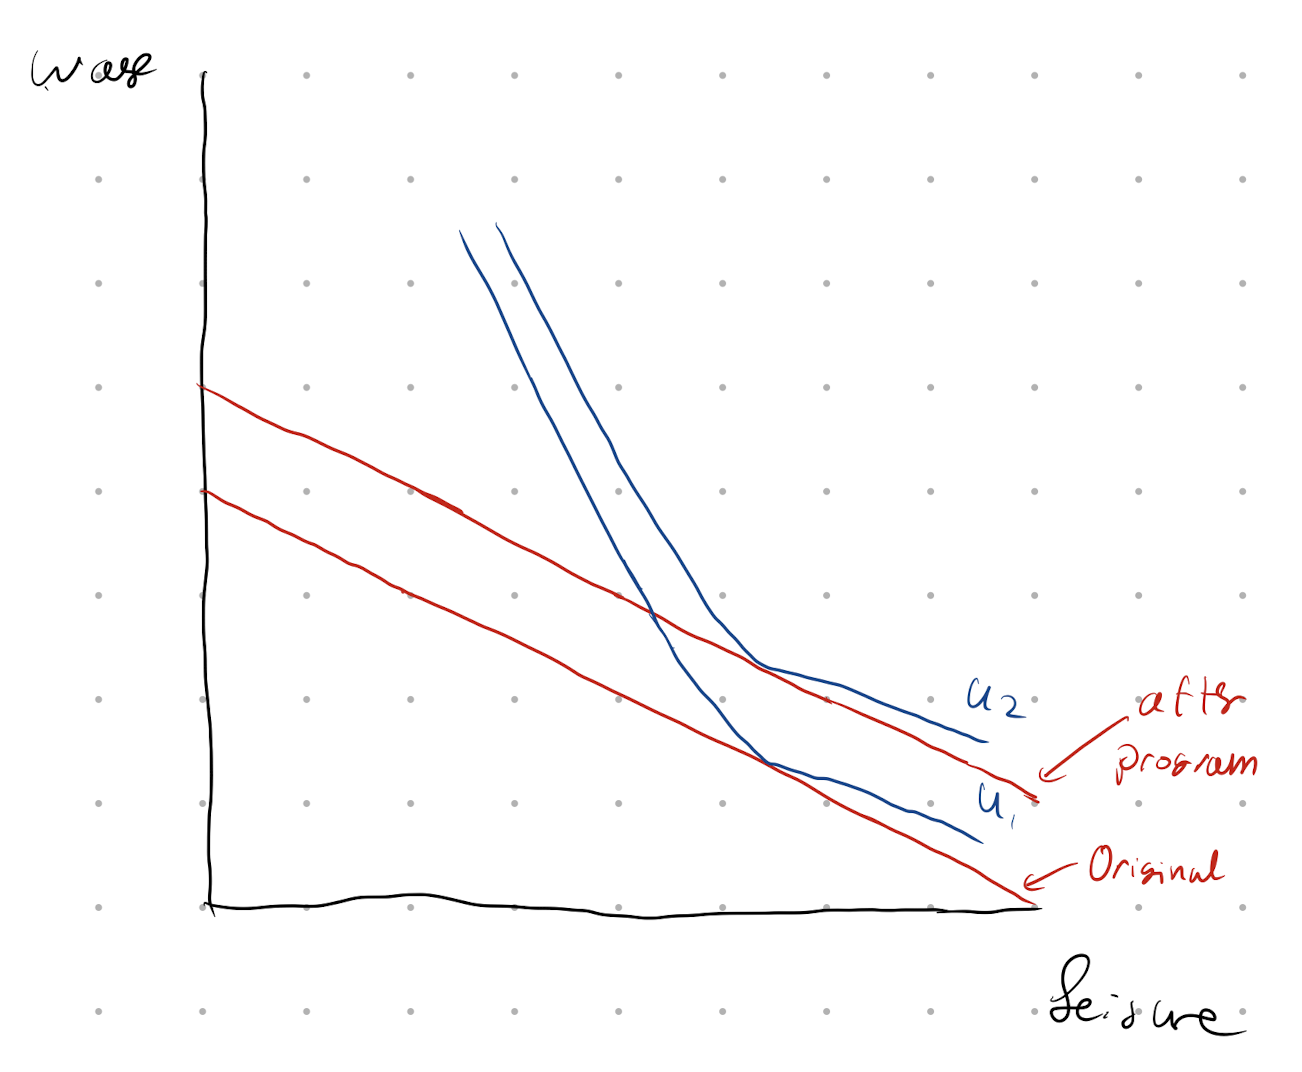
\includegraphics[width=10cm]{HW5Q3A}
\end{center}
\subsection*{Part B}
This is a universal basic income, where at every wage level (even zero income), a person earns additional income.
\subsection*{Part C}
This is a good policy because it includes nonworkers (which are nearly 50\% of the population) as well as having little in the way of changed preferences between work and leisure — the fact that a person has the same supplemental income regardless of their employment makes for a very simple policy.
}\end{document}
